% ======================================================================

Este Capítulo apresenta a fundamentação teórica que será usada nesta
dissertação. A~\autoref{cap:refteorico} apresenta um breve resumo dos
principais trabalhos relacionados ao assunto. A distribuição de
probabilidade beta e suas propriedades encontram-se
na~\autoref{cap:densbeta}. A~\autoref{cap:norta} apresenta o algoritmo
NORTA, que será usado para simular variáveis aleatórias beta
correlacionadas. A~\autoref{cap:betamodel} introduz o modelo de
regressão beta (univariado). Por fim, a~\autoref{cap:gof} apresenta
brevemente as medidas de bondade de ajuste usadas na comparação entre os
modelos.

\section{REVISÃO DA LITERATURA}
\label{cap:refteorico}

\section{DISTRIBUIÇÃO DE PROBABILIDADE BETA}
\label{cap:densbeta}

\begin{figure}[!htb]
  \centering
  \vspace{0.35cm}
  \setlength{\abovecaptionskip}{.0001pt}
  \caption{FUNÇÃO DE DISTRIBUIÇÃO BETA PARA DIFERENTES VALORES DE $\mu$
    COMBINADOS COM $\phi = (0,00001;~0,666;~4;~9;~23,99)$}
  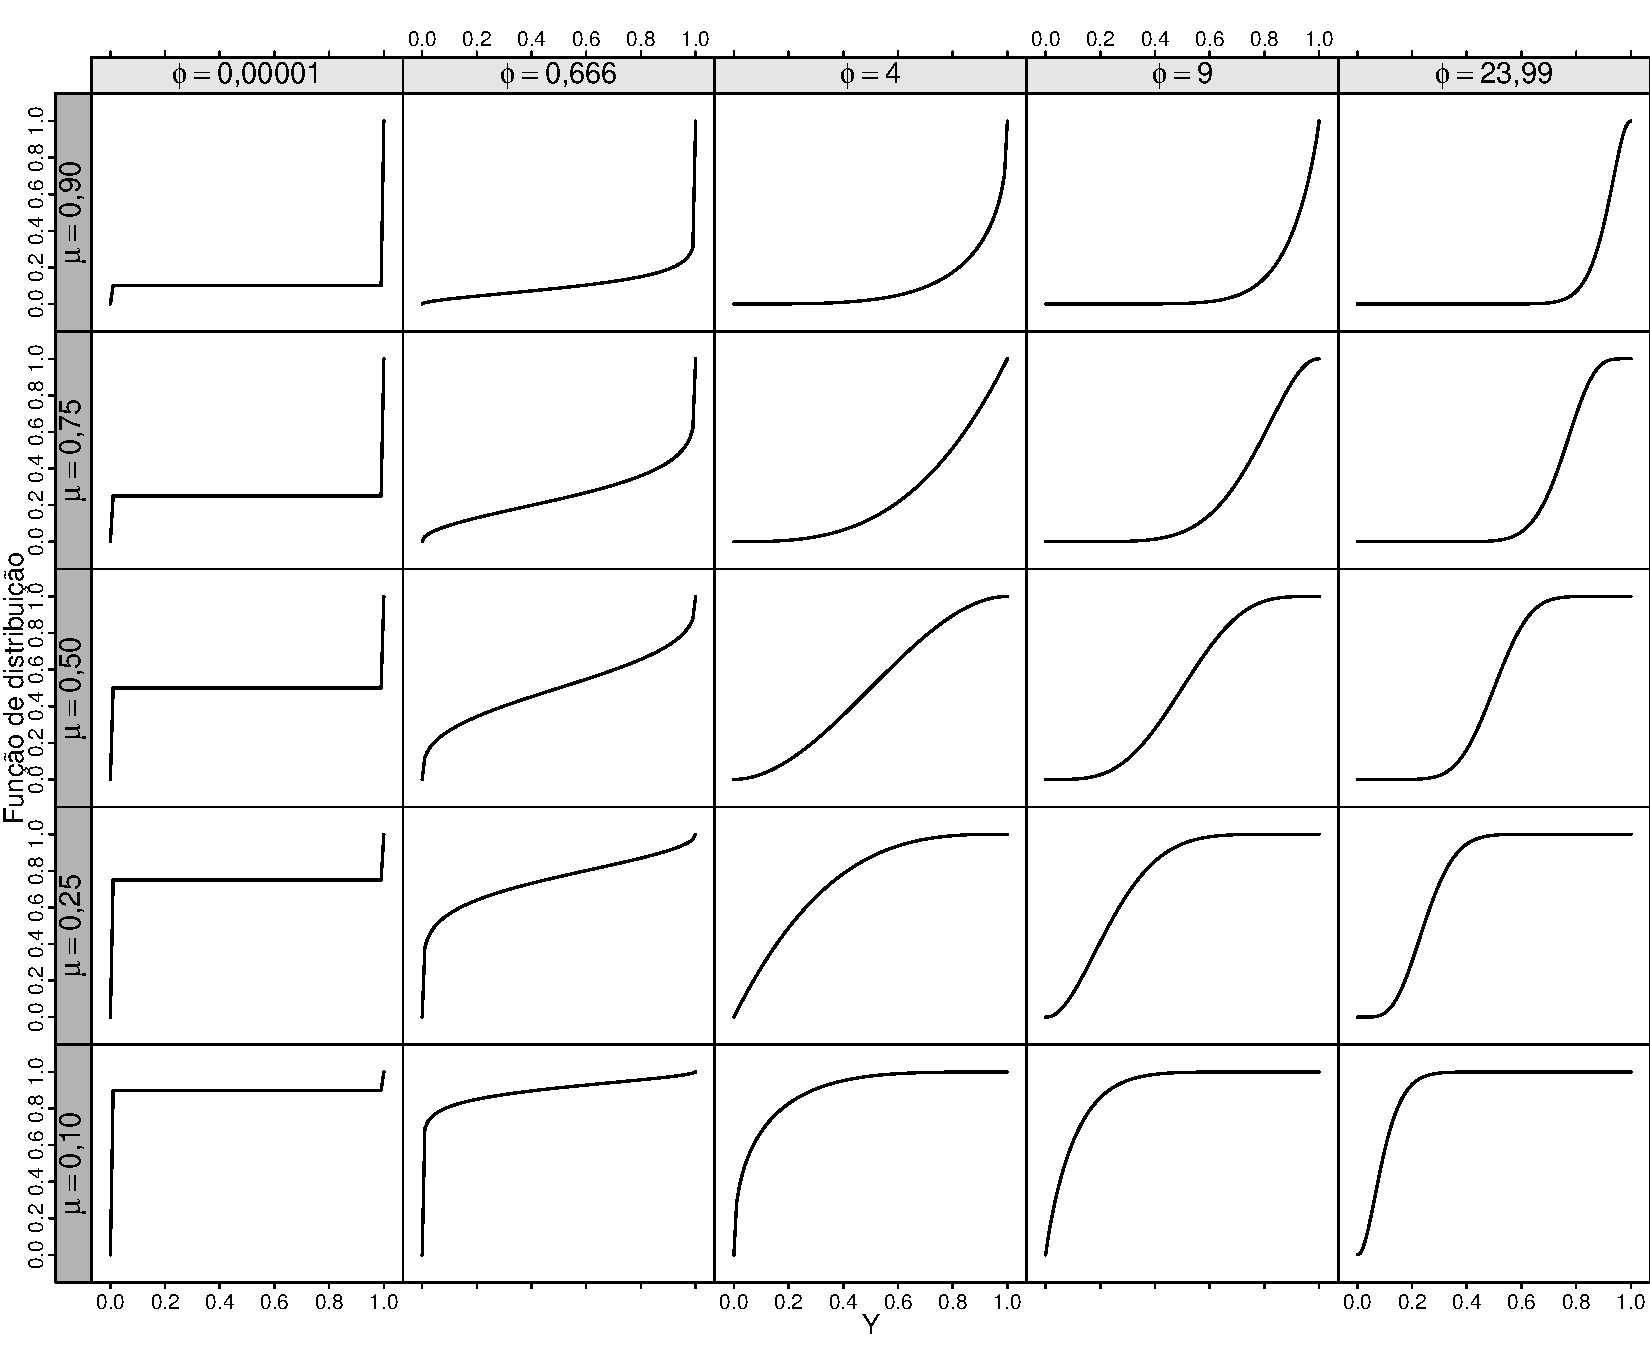
\includegraphics[width=.9\textwidth]{Figure6.pdf}
  \begin{footnotesize}
    \vspace{-0.1cm}
    FONTE: O autor~(2018).
    \vspace{0.15cm}
  \end{footnotesize}
  \label{fig:dbeta}
\end{figure}

\begin{figure}[H]
  \vspace{0.35cm}
  \setlength{\abovecaptionskip}{.00001pt}
  \caption{CÓDIGOS EM LINGUAGEM R PARA GERAÇÃO DE VARIÁVEIS ALEATÓRIAS
    BETA CORRELACIONADAS}
  \vspace{-0.5cm}
  \begin{program}[H]
    \begin{tikzpicture}
      \node [mybox] (box){
        \begin{minipage}{0.955\textwidth}
\begin{verbatim}
R = 1000  # tamanho da amostra
mu = 0.5  # parâmetro de média
phi = 9  # parâmetro de dispersão
cor_matrix <- matrix(c(1.0,0.75,0.75,1.0),2,2) # matriz de correlação
require(MASS)  # carrega o pacote com a função mvrnorm()
Z <- mvrnorm(n = R, mu = c(0,0), Sigma = cor_matrix)  # passo 1
Y <- qbeta(pnorm(Z), shape1 = mu*phi, shape2 = (1 - mu)*phi) # passo 2
\end{verbatim}
        \end{minipage}
      };
    \end{tikzpicture}
  \end{program}
  \vspace{-0.5cm}
  \begin{footnotesize}
    \centering
    FONTE: O autor~(2018).
    \vspace{-0.28cm}
  \end{footnotesize}
  \label{fig:steps1e2}
\end{figure}

% ======================================================================